% Build: module load texlive/20240312-GCC-13.3.0 && latexmk -pdf rebuild_talk.tex

\documentclass[11pt,aspectratio=169]{beamer}

% ---------------------------------------------------------------------------
% Look: plain beamer, Yale colours
% ---------------------------------------------------------------------------
\usetheme{default}
\usefonttheme{professionalfonts}
\setbeamertemplate{navigation symbols}{}

\definecolor{yaleblue}{HTML}{00356B}
\definecolor{yalemid}{HTML}{286DC0}
\definecolor{yalelight}{HTML}{63AAFF}
\definecolor{yalegrey}{HTML}{4A4A4A}
\definecolor{yalelightgrey}{HTML}{DDDDDD}

\setbeamercolor{structure}{fg=yaleblue}
\setbeamercolor{normal text}{fg=black}
\setbeamercolor{frametitle}{fg=yaleblue}
\setbeamercolor{title}{fg=yaleblue}
\setbeamercolor{alerted text}{fg=yalemid}
\setbeamercolor{block title}{fg=white,bg=yaleblue}
\setbeamercolor{block body}{bg=yalelightgrey!40}

\setbeamerfont{frametitle}{series=\bfseries,size=\large}
\setbeamerfont{title}{series=\bfseries,size=\Large}

\setbeamertemplate{itemize items}[circle]
\setbeamertemplate{blocks}[rounded][shadow=false]

% A thin blue rule under each frame title
\setbeamertemplate{frametitle}{%
  \vspace*{0.6em}%
  \usebeamerfont{frametitle}\usebeamercolor[fg]{frametitle}\insertframetitle\par
  \vspace*{-0.2em}{\color{yaleblue}\rule{\textwidth}{0.6pt}}%
}

% Footer: short title on the left, slide number on the right
\setbeamertemplate{footline}{%
  \hspace*{1.2em}{\color{yalegrey}\scriptsize\insertshorttitle}%
  \hfill{\color{yalegrey}\scriptsize\insertframenumber}\hspace*{1.2em}%
  \vspace*{0.6em}%
}

% ---------------------------------------------------------------------------
% Packages
% ---------------------------------------------------------------------------
\usepackage[T1]{fontenc}
\usepackage{lmodern}
\usepackage{booktabs}
\usepackage{array}
\usepackage{graphicx}
\usepackage{amsmath}
\usepackage{tikz}
\usetikzlibrary{positioning,arrows.meta,calc}
\usepackage{pgfplots}
\pgfplotsset{compat=1.18}
\graphicspath{{figures/}}

% Diagram styles
\tikzset{
  tok/.style={draw=yaleblue, rounded corners=2pt, font=\small, inner sep=4pt,
              minimum height=0.65cm},
  blank/.style={tok, fill=yalelight!35, font=\small\bfseries},
  box/.style={draw=yaleblue, rounded corners=2pt, font=\scriptsize, align=center,
               text width=2.1cm, minimum height=1.1cm, inner sep=3pt},
  arr/.style={-{Stealth[length=5pt]}, yaleblue, thick},
  cF/.style={fill=yaleblue},
  cP/.style={fill=yalelight!60},
  cN/.style={fill=white},
}

\pgfplotsset{colormap={yalemap}{color=(white) color=(yalelight) color=(yaleblue)}}


% Distribution maps (slides on pretraining and post-training): a smooth 2D
% density from Gaussian bumps g, shaded white to Yale blue.
\pgfplotsset{sentencemap/.style={view={0}{90}, width=6.6cm, height=5.4cm,
    xmin=-3, xmax=3, ymin=-3, ymax=3, ticks=none, colormap name=yalemap,
    axis line style={yalegrey}, clip=false,
    /pgf/declare function={g(\x,\y,\a,\b,\s) = exp(-((\x-\a)^2 + (\y-\b)^2)/(2*\s^2));}}}

% Four labelled points on a distribution map, at fixed positions:
% #1 top left, #2 top right, #3 bottom right, #4 bottom left (the unrealistic one)
\newcommand{\maplabels}[4]{%
  \begin{scope}[every node/.style={font=\tiny, fill=white, fill opacity=0.8,
        text opacity=1, inner sep=1.5pt, rounded corners=1pt, align=left}]
    \fill[black] (axis cs:-1.6,1.2,5) circle (1.2pt);
    \node[anchor=south west] at (axis cs:-1.7,1.3,5) {#1};
    \fill[black] (axis cs:1.4,1.3,5) circle (1.2pt);
    \node[anchor=north, align=center] at (axis cs:1.4,1.2,5) {#2};
    \fill[black] (axis cs:1.5,-1.5,5) circle (1.2pt);
    \node[anchor=north, align=center] at (axis cs:1.5,-1.6,5) {#3};
    \fill[black] (axis cs:-2.2,-2.4,5) circle (1.2pt);
    \node[anchor=south west] at (axis cs:-2.2,-2.3,5) {#4};
  \end{scope}}

\newcommand{\recordlabels}{\maplabels{married, 38,\\ two children}{age 81, Social\\ Security \$31k}{age 70, \$400k saved,\\ \$2k interest (0.5\%)}{age 9, wages \$300k}}

% Training slide. Cells sit at column #1, row #2 of a picture with x=1.5cm, y=0.85cm.
\tikzset{
  cell/.style={tok, minimum width=1.38cm, minimum height=0.7cm, font=\scriptsize},
  hid/.style={blank, minimum width=1.38cm, minimum height=0.7cm, font=\scriptsize\bfseries},
  absent/.style={cell, draw=yalelightgrey, fill=yalelightgrey!50, text=yalegrey},
}
\newcommand{\cellv}[3]{\node[cell] at (#1,-#2) {#3};}          % a visible value
\newcommand{\cellh}[2]{\node[hid] at (#1,-#2) {?};}            % a hidden cell
\newcommand{\cella}[2]{\node[absent] at (#1,-#2) {--};}        % not in this source
% A guessed distribution: #3 the bar heights (tallest = 1), #4 the true bar
% (0 = truth not shown yet), #5 the true value
\newcommand{\cellg}[5]{%
  \node[hid] at (#1,-#2) {};
  \foreach \hgt [count=\k] in {#3} {
    \ifnum\k=#4 \def\barcol{yaleblue}\else\def\barcol{yalemid!40}\fi
    \fill[\barcol] ($(#1,-#2)+(-0.75cm+\k*0.15cm,-0.27cm)$) rectangle ++(0.1cm,\hgt*0.5cm);
  }
  \ifnum#4>0 \node[font=\tiny, text=yaleblue] at ($(#1,-#2)+(0.4cm,0)$) {#5};\fi
}
% The network strip under the table: idle, guess (arrows on), or update (weights lit)
\newcommand{\trainnet}[1]{%
  \begin{scope}[shift={(5,-5.5)}, x=1cm, y=1cm]
    \def\mode{#1}\def\upd{update}\def\idle{idle}
    \ifx\mode\upd \def\wcol{yalemid}\def\wth{0.9pt}\else \def\wcol{yalelightgrey}\def\wth{0.4pt}\fi
    \foreach \a in {-0.5,-0.17,0.17,0.5} \foreach \b in {-0.5,-0.17,0.17,0.5} {
      \draw[\wcol, line width=\wth] (-0.8,\a) -- (0,\b);
      \draw[\wcol, line width=\wth] (0,\a) -- (0.8,\b);
    }
    \foreach \lx in {-0.8,0,0.8} \foreach \ly in {-0.5,-0.17,0.17,0.5}
      \fill[yaleblue] (\lx,\ly) circle (2.2pt);
    \ifx\mode\idle\else
      \draw[arr] (-3.2,0) -- (-1.1,0);
      \node[font=\scriptsize, anchor=south] at (-2.15,0.05) {visible cells};
      \draw[arr] (1.1,0) -- (2.9,0);
      \node[font=\scriptsize, anchor=south] at (2.0,0.05) {a guess for each ?};
    \fi
    \ifx\mode\upd \node[font=\scriptsize, text=yalemid, anchor=north] at (0,-0.6) {adjust the weights}; \fi
  \end{scope}}

% 100 squares, 10 by 10, at #1: the first #2 dark, the next #3 light, the rest
% empty; #4 a caption underneath
\newcommand{\waffle}[4]{%
  \begin{scope}[shift={(#1)}]
    \foreach \n in {0,...,99} {
      \pgfmathtruncatemacro{\col}{mod(\n,10)}
      \pgfmathtruncatemacro{\row}{div(\n,10)}
      \pgfmathtruncatemacro{\light}{#2+#3}
      \ifnum\n<#2 \def\wf{yaleblue}\else\ifnum\n<\light \def\wf{yalelight!70}\else\def\wf{white}\fi\fi
      \filldraw[fill=\wf, draw=yalegrey!60] (\col*0.32, -\row*0.32) rectangle ++(0.28,0.28);
    }
    \node[font=\small, anchor=north] at (1.58,-3.05) {#4};
  \end{scope}}

% Small grey note at the bottom of a slide
\newcommand{\slidenote}[1]{\par\vfill{\scriptsize\color{yalegrey}#1}}

% ---------------------------------------------------------------------------
% Title
% ---------------------------------------------------------------------------
\title{Using deep learning to generate synthetic tax records}
\author{John Ricco}
\institute{The Budget Lab at Yale}
\date{October 28, 2026}

% No hyphenation on slides
\hyphenpenalty=10000
\exhyphenpenalty=10000

\begin{document}

\begin{frame}[plain,noframenumbering]
  \titlepage
\end{frame}

% ===========================================================================
% 1. The problem
% ===========================================================================

\begin{frame}{What do we want?}
  \vfill
  \begin{center}
    {\LARGE\bfseries\color{yaleblue} Augmented tax unit microdata\\[0.3em] for every year, including future years}
  \end{center}
  \vfill
\end{frame}

\begin{frame}{What do we have?}
  \begin{itemize}
    \item \textbf{One year of tax data, filers only}
    \begin{itemize}
      \item About ten years out of date
      \item Some values are blurred and some records are distorted
      \item No non-filers, and none of the other variables a tax calculation needs:
            consumption, wealth, unrealized gains, estates
    \end{itemize}
    \vspace{0.5em}
    \item \textbf{Surveys} that hold some of this information, but noisily and not
          at administrative quality
    \vspace{0.5em}
    \item \textbf{Aggregate targets}
    \begin{itemize}
      \item Past years: IRS totals by AGI group, filing status and age range
      \item Future years: CBO-style projections of 1040 items, or of total wages,
            business profits and similar totals
    \end{itemize}
  \end{itemize}
\end{frame}

\begin{frame}{The task}
  \vfill
  \begin{center}
    {\Large Turn these scattered sources into\\[0.4em]
    {\bfseries\color{yaleblue} synthetic, realistic, augmented tax unit microdata}\\[0.4em]
    for every year}
  \end{center}
  \vfill
\end{frame}

% ===========================================================================
% 2. The traditional approach, built up one step at a time on a made-up table
% ===========================================================================

% Column centres (cm) of the picture: status, weight, wages, interest, capital
% gains from the PUF; net worth, consumption, tips imputed from surveys.
\def\cS{0.95}\def\cW{2.55}\def\cWg{3.85}\def\cI{5.15}\def\cG{6.45}
\def\cN{7.85}\def\cC{9.3}\def\cT{10.6}
\tikzset{
  tc/.style={draw=yalegrey!60, font=\scriptsize, minimum height=0.46cm, inner sep=1pt},
  tw/.style={tc, minimum width=#1},
  added/.style={fill=yalelight!25},
  imputed/.style={fill=yalemid!15},
  wup/.style={fill=wgreen!25, text=wgreen!70!black, font=\scriptsize\bfseries},
  wdown/.style={fill=wred!20, text=wred!80!black, font=\scriptsize\bfseries},
}
\definecolor{wgreen}{HTML}{2E8B57}
\definecolor{wred}{HTML}{C0392B}
% A record from the tax data: #1 row y, #2 extra style, then status, weight,
% wages, interest, capital gains
\newcommand{\pufrow}[7]{%
  \node[tw=1.9cm,#2] at (\cS,#1) {#3};
  \node[tw=1.3cm,#2] at (\cW,#1) {#4};
  \node[tw=1.3cm,#2] at (\cWg,#1) {#5};
  \node[tw=1.3cm,#2] at (\cI,#1) {#6};
  \node[tw=1.3cm,#2] at (\cG,#1) {#7};}
% The imputed columns of a record: #1 row y, then net worth, consumption, tips
\newcommand{\improw}[4]{%
  \node[tw=1.5cm,imputed] at (\cN,#1) {#2};
  \node[tw=1.4cm,imputed] at (\cC,#1) {#3};
  \node[tw=1.2cm,imputed] at (\cT,#1) {#4};}
% A reweighted weight: #1 row y, #2 the new weight, higher or lower
\newcommand{\wupcell}[2]{\node[tw=1.3cm,wup] at (\cW,#1) {#2 $\uparrow$};}
\newcommand{\wdncell}[2]{\node[tw=1.3cm,wdown] at (\cW,#1) {#2 $\downarrow$};}

\begin{frame}{How has this been done before?}
  \centering
  \begin{tikzpicture}[x=1cm, y=1cm]
    \useasboundingbox (-2.6,0.55) rectangle (11.3,-4.75);

    % header
    \foreach \x/\lab in {\cS/Status, \cW/Weight, \cWg/Wages, \cI/Interest, \cG/{Capital\\gains}}
      \node[font=\scriptsize\bfseries, text=yaleblue, align=center, anchor=south, text depth=0.4ex] at (\x,-0.3) {\lab};

    % filers from the PUF
    \pufrow{-1.15}{}{Married}{812}{\$142k}{\$310}{\$5.2k}
    \pufrow{-1.61}{}{Single}{1,404}{\$38k}{\$0}{\$0}
    \pufrow{-2.07}{}{Married}{655}{\$0}{\$4.9k}{\$61k}
    \pufrow{-2.53}{}{Head of hh.}{1,120}{\$51k}{\$12}{\$0}
    \pufrow{-2.99}{}{Single}{3}{\$2.3m}{\$88k}{\$3.9m}
    \node[font=\scriptsize, anchor=east, align=right] at (-0.15,-2.07) {Filers\\(PUF)};

    % step 2: records added above and below
    \onslide<2->{
      \pufrow{-0.5}{added}{Married}{1}{\$1.2m}{\$14m}{\$310m}
      \node[font=\scriptsize, anchor=east, align=right] at (-0.15,-0.5) {Billionaires};
      \pufrow{-3.65}{added}{Single}{2,310}{\$0}{\$0}{\$0}
      \pufrow{-4.11}{added}{Single}{1,870}{\$6.5k}{\$0}{\$0}
      \node[font=\scriptsize, anchor=east, align=right] at (-0.15,-3.88) {Non-filers};
    }

    % step 3: columns added on the right
    \onslide<3->{
      \foreach \x/\lab in {\cN/{Net\\worth}, \cC/{Consump-\\tion}, \cT/Tips}
        \node[font=\scriptsize\bfseries, text=yalemid, align=center, anchor=south, text depth=0.4ex] at (\x,-0.3) {\lab};
      \improw{-0.5}{\$4.1b}{\$6m}{\$0}
      \improw{-1.15}{\$610k}{\$96k}{\$0}
      \improw{-1.61}{\$9k}{\$34k}{\$6.1k}
      \improw{-2.07}{\$2.4m}{\$88k}{\$0}
      \improw{-2.53}{\$31k}{\$47k}{\$0}
      \improw{-2.99}{\$38m}{\$410k}{\$0}
      \improw{-3.65}{\$2k}{\$19k}{\$0}
      \improw{-4.11}{\$1k}{\$15k}{\$1.2k}
    }

    % step 4: weights move up or down
    \only<4>{
      \wupcell{-1.15}{860}
      \wdncell{-1.61}{1,290}
      \wupcell{-2.07}{702}
      \wupcell{-2.53}{1,180}
      \wdncell{-2.99}{2}
      \wupcell{-3.65}{2,450}
      \wdncell{-4.11}{1,760}
    }
  \end{tikzpicture}

  \vspace{0.5em}
  \small
  \only<1>{\textbf{1. Start with the IRS PUF}, whatever year is available.}%
  \only<2>{\textbf{2. Add records}: non-filers, and the very rich the PUF leaves out.}%
  \only<3>{\textbf{3. Add columns}: estimate $Y$ given $X$ in a survey, where $X$ is also on the PUF; draw $Y$ for each record.}%
  \only<4>{\textbf{4. Reweight to the target year}: grow weights for population and dollars for prices,
           then move each weight up or down until the year's totals are hit.}
  \slidenote{Made-up records.}
\end{frame}

\begin{frame}{What were the problems with this approach?}
  \begin{itemize}
    \item \textbf{It did not work well for past years.} The affordability project made this clear.
    \vspace{0.6em}
    \item \textbf{A separate model for each variable}, each estimating its conditional
          relationships in its own way.
    \vspace{0.6em}
    \item \textbf{Reweighting worked for only a few past years.} Tax law changed what the
          IRS targets measure, mainly TCJA cutting back itemized deductions.
    \vspace{0.6em}
    \item \textbf{Stretched further every year.} Plausible records for future years, but
          worse with each year away from 2015.
  \end{itemize}
\end{frame}

\begin{frame}{The ideal approach}
  \begin{enumerate}
    \item Take in survey data covering the joint relationships among every variable we
          might want to model.
    \vspace{0.6em}
    \item Learn all of those relationships in \textbf{One Huge Joint Probability Distribution}.
    \vspace{0.6em}
    \item For any target year, supply the targets that describe that year, and pull out
          of it the records that match them.
  \end{enumerate}
  \vspace{1em}
  The result: a realistic synthetic microdata set for that year.
  \slidenote{From a conversation with John and Harris.}
\end{frame}

% ===========================================================================
% 3. The analogy to language models (maps from the 21 October deck)
% ===========================================================================

\begin{frame}{Language models: pretraining, then post-training}
  \centering
  \begin{tikzpicture}
    \begin{axis}[sentencemap, name=pre, title={\small\bfseries Pretraining}]
      \addplot3[surf, shader=interp, samples=45, domain=-3:3, y domain=-3:3]
        {1.0*g(x,y,-1.6,1.2,0.8) + 0.8*g(x,y,1.4,1.3,0.7) + 0.6*g(x,y,1.5,-1.5,0.6)
         + 0.9*g(x,y,-0.6,-0.9,0.9) + 0.5*g(x,y,0.3,0.3,0.7)};
      \maplabels{`The cat sat on the mat.'}{`Sure! Let me look\\ at your code first.'}{`The way to make\\ a bomb is'}{`mat the on cat sat'}
    \end{axis}
    \begin{axis}[sentencemap, at={($(pre.east)+(0.8cm,0)$)}, anchor=west,
        title={\small\bfseries Post-training}]
      \addplot3[surf, shader=interp, samples=45, domain=-3:3, y domain=-3:3]
        {0.2*g(x,y,-1.6,1.2,0.8) + 3.0*g(x,y,1.4,1.3,0.7) + 0.005*g(x,y,1.5,-1.5,0.6)
         + 0.2*g(x,y,-0.6,-0.9,0.9) + 0.2*g(x,y,0.3,0.3,0.7)};
      \maplabels{`The cat sat on the mat.'}{`Sure! Let me look\\ at your code first.'}{`The way to make\\ a bomb is'}{`mat the on cat sat'}
    \end{axis}
  \end{tikzpicture}

  \vspace{0.3em}
  \begin{columns}[T]
    \begin{column}{0.45\textwidth}\centering\small
      Read the whole internet and learn which sentences are likely: a prior over language
    \end{column}
    \begin{column}{0.45\textwidth}\centering\small
      Squeeze the mass toward a helpful, harmless assistant, and away from nonsense and harm
    \end{column}
  \end{columns}
\end{frame}

\begin{frame}{Our model: pretraining, then post-training}
  \centering
  \begin{tikzpicture}
    \begin{axis}[sentencemap, name=pre, title={\small\bfseries Pretraining}]
      \addplot3[surf, shader=interp, samples=45, domain=-3:3, y domain=-3:3]
        {1.0*g(x,y,-1.6,1.2,0.8) + 0.8*g(x,y,1.4,1.3,0.7) + 0.6*g(x,y,1.5,-1.5,0.6)
         + 0.9*g(x,y,-0.6,-0.9,0.9) + 0.5*g(x,y,0.3,0.3,0.7)};
      \recordlabels
    \end{axis}
    \begin{axis}[sentencemap, at={($(pre.east)+(0.8cm,0)$)}, anchor=west,
        title={\small\bfseries Post-training for 2040}]
      \addplot3[surf, shader=interp, samples=45, domain=-3:3, y domain=-3:3]
        {0.5*g(x,y,-1.6,1.2,0.8) + 2.5*g(x,y,1.4,1.3,0.7) + 0.03*g(x,y,1.5,-1.5,0.6)
         + 0.6*g(x,y,-0.6,-0.9,0.9) + 0.5*g(x,y,0.3,0.3,0.7)};
      \recordlabels
    \end{axis}
  \end{tikzpicture}

  \vspace{0.3em}
  \begin{columns}[T]
    \begin{column}{0.45\textwidth}\centering\small
      Learn which records are likely, from every source: a prior over records
    \end{column}
    \begin{column}{0.45\textwidth}\centering\small
      Squeeze the mass toward records that hit 2040's totals, each still coherent
    \end{column}
  \end{columns}
  \vfill
  {\small Post-training finds the distribution closest to the prior that hits the year's totals.}
  \vspace{0.4em}
\end{frame}

% ===========================================================================
% 4. The method
% ===========================================================================

% Variant A of the method section: generation first.
% Horizontal probability bars at the origin: #1 a list of label/probability/drawn (1 = the drawn value).
\newcommand{\hbars}[1]{%
  \foreach \lab/\p/\d [count=\i] in {#1} {
    \ifnum\d=1 \def\bc{yaleblue}\def\tf{\bfseries}\else\def\bc{yalemid!35}\def\tf{}\fi
    \node[anchor=east, font=\scriptsize\tf] at (-0.05,-\i*0.42) {\lab};
    \fill[\bc] (0,-\i*0.42-0.14) rectangle ++(\p*5.5,0.28);
    \node[anchor=west, font=\scriptsize\tf] at (\p*5.5+0.05,-\i*0.42) {\p};
  }}
% One row of the record being written: #1 row number, #2 item, #3 value, #4 the slide it is drawn on
\newcommand{\recrow}[4]{%
  \onslide<#4->{
    \node[anchor=east, font=\scriptsize, text=yalegrey] at (2.0,-#1*0.32) {#2};
    \node[anchor=west, font=\scriptsize, inner sep=1.5pt, rounded corners=1pt,
          fill=yalelight!0] at (2.1,-#1*0.32) {#3};
    \only<#4>{\node[anchor=west, font=\scriptsize, inner sep=1.5pt, rounded corners=1pt,
          fill=yalelight!45] at (2.1,-#1*0.32) {#3};}
  }}

\begin{frame}{Writing one record, one item at a time}
  \begin{tikzpicture}
    \useasboundingbox (-0.2,0.6) rectangle (14.3,-5.0);
    % the record so far
    \node[anchor=west, font=\small\bfseries, text=yaleblue] at (0,0.3) {The record so far};
    \recrow{1}{source}{PUF}{1}
    \recrow{2}{year}{2015}{1}
    \recrow{3}{filer}{yes}{1}
    \recrow{4}{AGI group}{75th--90th percentile}{1}
    \recrow{5}{married}{yes}{2}
    \recrow{6}{dependents}{2}{3}
    \recrow{7}{age range}{35--44}{4}
    \recrow{8}{filing status}{joint}{5}
    \recrow{9}{credit children}{2 and 2}{5}
    \recrow{10}{wages}{82nd--84th pct.\ band}{6}
    \recrow{11}{interest}{zero}{7}
    \recrow{12}{dividends}{40th--42nd pct.\ band}{7}
    \recrow{13}{Schedule C}{zero}{7}
    \recrow{14}{\dots}{about 90 tax items}{7}
    \draw[yalelightgrey] (4.9,0.4) -- (4.9,-4.8);

    % what the model returns at this step
    \begin{scope}[shift={(6.6,0)}]
      \only<1>{
        \node[anchor=north west, text width=7.3cm, font=\small] at (-1.3,0.4)
          {We set four things before any draw:\\[0.4em]
           \begin{itemize}
             \item the source the record is written as (the PUF),
             \item its year (2015),
             \item that it is a filer,
             \item its AGI group, one of 12.
           \end{itemize}
           \vspace{0.4em}
           Then we ask the model for the next item.};
      }
      \only<2>{
        \node[anchor=west, font=\small\bfseries, text=yaleblue] at (-1.3,0.3) {Next: married?};
        \begin{scope}[shift={(0,-0.3)}]\hbars{no/0.31/0, yes/0.69/1}\end{scope}
      }
      \only<3>{
        \node[anchor=west, font=\small\bfseries, text=yaleblue] at (-1.3,0.3) {Next: dependents?};
        \begin{scope}[shift={(0,-0.3)}]\hbars{0/0.27/0, 1/0.22/0, 2/0.33/1, 3+/0.18/0}\end{scope}
      }
      \only<4>{
        \node[anchor=west, font=\small\bfseries, text=yaleblue] at (-1.3,0.3) {Next: age range?};
        \begin{scope}[shift={(0,-0.3)}]\hbars{under 26/0.01/0, 26--34/0.15/0, 35--44/0.36/1, 45--54/0.29/0, 55--64/0.14/0, 65+/0.05/0}\end{scope}
      }
      \only<5>{
        \node[anchor=north west, text width=7.3cm, font=\small] at (-1.3,0.4)
          {Then filing status and the number of child credit and EITC children, drawn the same way.\\[0.6em]
           Some draws follow rules: a married unit is always a joint return, as the PUF codes it.};
      }
      \only<6>{
        \node[anchor=west, font=\small\bfseries, text=yaleblue] at (-1.3,0.3) {Next: wages?};
        % zero band, then the 73 positive bands (bands, not dollars, on the axis)
        \fill[yalemid!35] (-1.0,-2.6) rectangle ++(0.1,0.25);
        \foreach \b in {1,...,73} {
          \pgfmathsetmacro{\hgt}{1.9*exp(-((\b-43)/6)^2) + 0.15*exp(-((\b-28)/12)^2)}
          \ifnum\b=42 \def\bc{yaleblue}\else\def\bc{yalemid!35}\fi
          \fill[\bc] (-0.75+\b*0.08,-2.6) rectangle ++(0.06,\hgt);
        }
        \draw[yalegrey] (-1.1,-2.6) -- (5.2,-2.6);
        \foreach \x/\lab in {-0.95/zero, 1.33/p50, 2.93/p90, 3.65/p99, 4.37/p99.9} {
          \draw[yalegrey] (\x,-2.6) -- ++(0,-0.08);
          \node[font=\tiny, anchor=north] at (\x,-2.66) {\lab};
        }
        \node[anchor=north west, text width=7.3cm, font=\small] at (-1.3,-3.2)
          {One bar for zero and 73 for positive wages, cut at percentiles of wage earners.
           Drawn (dark): the band from the 82nd to the 84th percentile.};
      }
      \only<7>{
        \node[anchor=north west, text width=7.3cm, font=\small] at (-1.3,0.4)
          {Every other tax item the same way, in a random order: each draw given
           everything drawn so far.\\[0.6em]
           Totals are never drawn. Capital gains, business income, ordinary
           dividends and the adjustments are added up from their drawn parts.\\[0.6em]
           Next: the items the PUF does not have.};
      }
    \end{scope}
  \end{tikzpicture}
  \slidenote{Made-up record and probabilities.}
\end{frame}

\begin{frame}{The rest of the record: what each survey would have recorded}
  \footnotesize
  Then the model is asked about the same unit as each survey would see it: the source label is
  switched, and the items that survey lacks are hidden from the model.

  \vspace{0.4em}
  \centering\footnotesize
  \renewcommand{\arraystretch}{1.2}
  \begin{tabular}{@{}>{\raggedright}p{2.0cm} >{\raggedright}p{5.6cm} >{\raggedright\arraybackslash}p{6.2cm}@{}}
    \toprule
    \textbf{Asked as} & \textbf{Draws} & \textbf{Sees, besides this phase's draws so far} \\
    \midrule
    CPS 2019 & exact ages of filer and spouse & the items the CPS shares with the PUF \\
    SCF, its wave & 20 balance-sheet items, unrealized gains & income items the SCF shares, exact ages \\
    CEX 2019 & 8 consumption categories & married, dependents, ages, wages, Social Security, self-employment income \\
    CPS 2019 & sex, dependents' ages, spouse's share of wages, weeks and hours, childcare & the items the CPS shares with the PUF, exact ages \\
    SIPP 2019 & each adult's tips, as a share of wages & married, dependents, ages, wages, spouse's share \\
    \bottomrule
  \end{tabular}

  \vspace{0.5em}
  \raggedright\small
  \begin{itemize}\setlength{\itemsep}{0pt}
    \item Each record's SCF wave is drawn at random: 2019 (55\%), 2022 (33\%), 2016 (12\%).
    \item Rules: mortgage interest on the return means a home and a mortgage; a dependent filer
          gets no survey items.
  \end{itemize}
\end{frame}

\begin{frame}{What one step returns, and how it becomes dollars}
  \begin{columns}[T]
    \begin{column}{0.48\textwidth}
      \textbf{\color{yaleblue}A probability for every possible value}
      \small
      \begin{itemize}\setlength{\itemsep}{3pt}
        \item A category (married, dependents 0--3, age range): one per value.
        \item An amount: one for each of 84 bands.
        \begin{itemize}
          \item exactly zero
          \item 10 bands of losses
          \item 73 bands of positive amounts, by percentile among holders: 2 points wide up
                to the 90th, then 1, 0.1 and 0.01 at the very top
        \end{itemize}
        \item No functional form: a spike at zero or a long top tail costs nothing extra.
      \end{itemize}
    \end{column}
    \begin{column}{0.48\textwidth}
      \textbf{\color{yaleblue}Bands become dollars at the end}
      \small
      \begin{itemize}\setlength{\itemsep}{3pt}
        \item Each band becomes one real value from that band, picked at random: from 2015
              PUF returns for tax items, the record's SCF wave for wealth, the 2019 CEX for spending.
        \item Then grown to 2019 item by item (tax items: SOI's growth in dollars per return
              with the item).
        \item Example: wages band 82nd--84th percentile; a real 2015 wage in it, \$96,400;
              grown to 2019, \$108,000.
      \end{itemize}
    \end{column}
  \end{columns}
  \slidenote{Example dollar amounts are made up.}
\end{frame}

\begin{frame}{Where the probabilities come from: training}
  \centering
  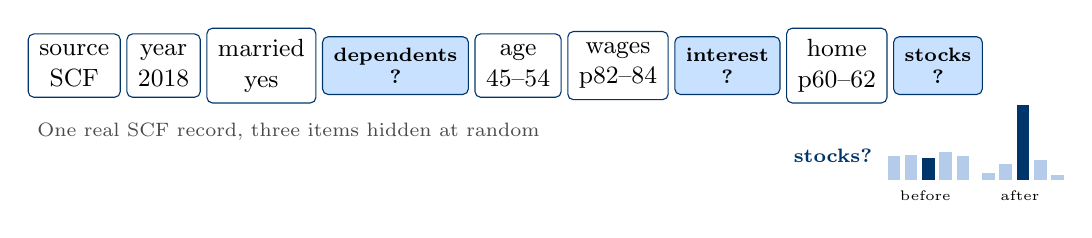
\begin{tikzpicture}
    \begin{scope}[every node/.append style={align=center, font=\scriptsize, inner sep=3pt,
                                            minimum height=0.95cm}]
      \node[tok, anchor=west] (r1) at (0,0) {source\\SCF};
      \node[tok, right=2pt of r1] (r2) {year\\2018};
      \node[tok, right=2pt of r2] (r3) {married\\yes};
      \node[blank, right=2pt of r3, font=\scriptsize\bfseries] (r4) {dependents\\?};
      \node[tok, right=2pt of r4] (r5) {age\\45--54};
      \node[tok, right=2pt of r5] (r6) {wages\\p82--84};
      \node[blank, right=2pt of r6, font=\scriptsize\bfseries] (r7) {interest\\?};
      \node[tok, right=2pt of r7] (r8) {home\\p60--62};
      \node[blank, right=2pt of r8, font=\scriptsize\bfseries] (r9) {stocks\\?};
    \end{scope}
    \node[anchor=north west, font=\scriptsize, text=yalegrey] at (0,-0.6)
      {One real SCF record, three items hidden at random};
    % the model's answer for one hidden item, before and after training
    \begin{scope}[shift={(10.9,0.15)}]
      \node[font=\scriptsize\bfseries, text=yaleblue, anchor=east] at (-0.05,-1.3) {stocks?};
      \foreach \h [count=\k] in {0.30,0.32,0.28,0.35,0.30} {
        \ifnum\k=3 \def\bc{yaleblue}\else\def\bc{yalemid!35}\fi
        \fill[\bc] (\k*0.22-0.2,-1.6) rectangle ++(0.16,\h);
      }
      \node[font=\tiny, anchor=north] at (0.5,-1.62) {before};
      \foreach \h [count=\k] in {0.08,0.20,0.95,0.25,0.06} {
        \ifnum\k=3 \def\bc{yaleblue}\else\def\bc{yalemid!35}\fi
        \fill[\bc] (\k*0.22+1.0,-1.6) rectangle ++(0.16,\h);
      }
      \node[font=\tiny, anchor=north] at (1.7,-1.62) {after};
    \end{scope}
  \end{tikzpicture}

  \vspace{0.2em}
  \raggedright\small
  \begin{enumerate}\setlength{\itemsep}{1pt}
    \item On each real record, from all five sources, hide anywhere from one to all of its items.
          Source and year stay shown.
    \item The model returns probabilities for each hidden item.
    \item Adjust its 1.4 million parameters to raise the probability on the true values
          (maximum likelihood, by survey weight; top records count extra). 80 passes over all records.
  \end{enumerate}
  \vspace{0.2em}
  Any set can be hidden, so one model answers ``this item, given any others'': what each
  step of writing a record asks.
  \slidenote{Made-up record and probabilities. The dark bar is the record's true band.}
\end{frame}

\begin{frame}{Post-training: reweight to hit the totals}
  \begin{columns}[T]
    \begin{column}{0.44\textwidth}
      \small
      \begin{enumerate}\setlength{\itemsep}{4pt}
        \item Draw 400,000 filers, a set number per AGI group, and non-filers
              as the CPS 2019 would see them.
        \item Start each weight at its AGI group's 2015 returns over the records drawn in it.
        \item Move the weights as little as possible (as in entropy balancing) until each of
              2019's 753 targets is within one standard error (SCF targets: half).
      \end{enumerate}
      \vspace{0.2em}
      The records do not change, only their weights.
    \end{column}
    \begin{column}{0.54\textwidth}
      \centering
      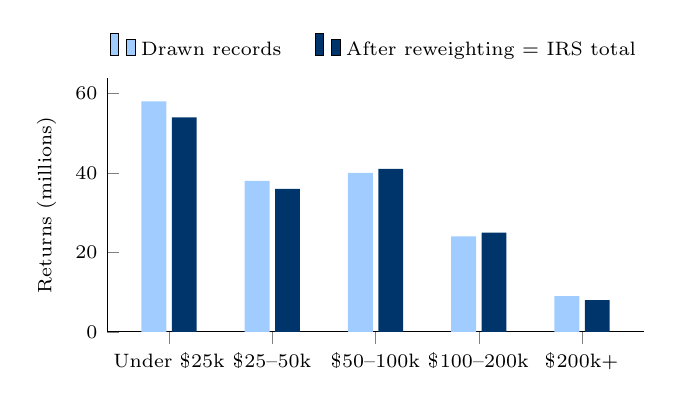
\begin{tikzpicture}
        \begin{axis}[ybar, width=8.4cm, height=4.8cm, bar width=9pt, ymin=0,
            symbolic x coords={Under \$25k, \$25--50k, \$50--100k, \$100--200k, \$200k+},
            xtick=data, xticklabel style={font=\scriptsize}, ylabel={Returns (millions)},
            ylabel style={font=\scriptsize}, yticklabel style={font=\scriptsize},
            legend style={font=\scriptsize, draw=none, at={(0.5,1.03)}, anchor=south, legend columns=2,
                          /tikz/every even column/.append style={column sep=1em}},
            axis x line*=bottom, axis y line*=left, enlarge x limits=0.15]
          \addplot[fill=yalelight!60, draw=none] coordinates
            {(Under \$25k,58) (\$25--50k,38) (\$50--100k,40) (\$100--200k,24) (\$200k+,9)};
          \addplot[fill=yaleblue, draw=none] coordinates
            {(Under \$25k,54) (\$25--50k,36) (\$50--100k,41) (\$100--200k,25) (\$200k+,8)};
          \legend{Drawn records, After reweighting = IRS total}
        \end{axis}
      \end{tikzpicture}
    \end{column}
  \end{columns}
  \slidenote{Made-up numbers in the chart.}
\end{frame}

% ===========================================================================
% 5. Challenges. Interest numbers: 2016 SCF (tax year 2015) against the 2015 PUF,
% weighted, married with wages $75k-200k (21 October deck; source report in
% rebuild/explore/2026-10-21/reporting_formula/, as cited there).
% ===========================================================================

\begin{frame}{Challenge: surveys and returns measure differently}
  \centering
  \begin{tikzpicture}
    \begin{axis}[ybar, width=12cm, height=5.4cm, bar width=14pt, ymin=0, ymax=32,
        symbolic x coords={\$1--100, \$100--500, \$500--2k, \$2k--10k, \$10k+},
        xtick=data, xticklabel style={font=\small}, yticklabel style={font=\small},
        ylabel={Per 100 tax units}, ylabel style={font=\small},
        xlabel={Interest received in the year}, xlabel style={font=\small},
        legend style={font=\small, draw=none, at={(0.97,0.95)}, anchor=north east},
        axis x line*=bottom, axis y line*=left, enlarge x limits=0.12,
        nodes near coords, every node near coord/.append style={font=\scriptsize}]
      \addplot[fill=yaleblue, draw=none] coordinates
        {(\$1--100,28) (\$100--500,13) (\$500--2k,4) (\$2k--10k,2) (\$10k+,1)};
      \addplot[fill=yalelight!70, draw=none] coordinates
        {(\$1--100,8) (\$100--500,6) (\$500--2k,3) (\$2k--10k,3) (\$10k+,1)};
      \legend{PUF: on the return (48 in all), SCF: say they have it (21 in all)}
    \end{axis}
  \end{tikzpicture}

  \vspace{0.3em}
  The gap is all in small amounts: they go unreported in the survey. Above \$2,000 the two sources agree.
  \slidenote{Married, wages \$75--200k. 2015 PUF and 2016 SCF (tax year 2015), weighted.}
\end{frame}

\begin{frame}{The fix: two slots and a fill-in}
  \begin{columns}[c]
    \begin{column}{0.5\textwidth}
      \centering
      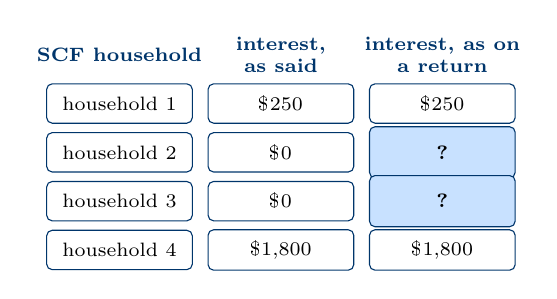
\begin{tikzpicture}[x=2.05cm, y=0.62cm,
          c/.style={tok, minimum width=1.85cm, minimum height=0.5cm, font=\scriptsize}]
        \node[font=\scriptsize\bfseries, text=yaleblue] at (1,0) {SCF household};
        \node[font=\scriptsize\bfseries, text=yaleblue, align=center] at (2,0) {interest,\\as said};
        \node[font=\scriptsize\bfseries, text=yaleblue, align=center] at (3,0) {interest, as on\\a return};
        \foreach \r/\said/\ret/\hd in {1/\$250/\$250/0, 2/\$0/?/1, 3/\$0/?/1, 4/{\$1,800}/{\$1,800}/0} {
          \node[c] at (1,-\r) {household \r};
          \node[c] at (2,-\r) {\said};
          \ifnum\hd=1 \node[c, blank, font=\scriptsize\bfseries] at (3,-\r) {\ret}; \else \node[c] at (3,-\r) {\ret}; \fi
        }
      \end{tikzpicture}

      \vspace{0.8em}
      \small
      The answer given is kept. A second slot holds what the return would show,
      the only slot the PUF has.
    \end{column}
    \begin{column}{0.46\textwidth}
      \centering
      \small
      \begin{tabular}{lrrr}
        \toprule
        Per 100 couples & PUF & SCF & Fill in \\
        \midrule
        \$1--100      & 28 & 8 & 20 \\
        \$100--500    & 13 & 6 & 7 \\
        \$500--2k     & 4  & 3 & 2 \\
        \$2k and over & 3  & 3 & 0 \\
        \midrule
        Any           & 48 & 21 & 28 \\
        \bottomrule
      \end{tabular}

      \vspace{0.8em}
      The PUF sets how many are filled in, and at what sizes.
      The rest of the SCF record sets which households.
    \end{column}
  \end{columns}
  \slidenote{Married, wages \$75--200k. 2015 PUF and 2016 SCF (tax year 2015), weighted. Rows may not add because of rounding.}
\end{frame}

\begin{frame}{Other challenges}
  \begin{itemize}
    \item \textbf{Building tax units from surveys.} Surveys count households. Each one is split
          into tax units by the same rules for every survey, and then we decide who files.
    \vspace{0.5em}
    \item \textbf{The return itself changes.} TCJA cut back itemizing; new items, like the
          tips and overtime deductions, are on no past return.
    \vspace{0.5em}
    \item \textbf{A thin top.} Few very rich records in any source.
    \vspace{0.5em}
    \item \textbf{Future years.} No microdata, only a handful of projected totals.
    \vspace{0.5em}
    \item \textbf{Checking the result.} No source has every variable, so some relationships
          have nothing to check against.
  \end{itemize}
\end{frame}

% ===========================================================================
% 6. Where we are
% ===========================================================================

\begin{frame}{Where we are}
  \begin{itemize}
    \item A 2019 file: 400,000 filer records, plus non-filers
    \vspace{0.4em}
    \item Five sources: the 2015 PUF, the SCF, the CEX, the CPS and the SIPP, every survey
          split into tax units by the same rules
    \vspace{0.4em}
    \item Every PUF item, plus a balance sheet, consumption, tips and auto loan interest
    \vspace{0.4em}
    \item About 750 targets, all met within their standard errors: IRS tables by AGI,
          filing status and age, the top 1\%, 0.1\% and 0.01\%, W-2 tips, SCF wealth
  \end{itemize}
\end{frame}

\begin{frame}{What is left}
  \begin{itemize}
    \item Rules applied after drawing: credit eligibility, death probabilities, unrealized gains,
          the basis of capital gains
    \vspace{0.4em}
    \item The file Tax-Simulator reads, and a first run of Tax-Simulator on it
    \vspace{0.4em}
    \item A tax calculator inside post-training, for targets on computed tax
    \vspace{0.4em}
    \item Other years: 2015 to 2023, then the projection years
    \vspace{0.4em}
    \item The very top: the PUF's aggregate records and the Forbes 400
  \end{itemize}
\end{frame}

\begin{frame}[plain,noframenumbering,c]
  \begin{center}
    {\color{yaleblue}\Large\bfseries Questions}
  \end{center}
\end{frame}

% ---------------------------------------------------------------------------
% Parked: the 24 October intro slides, kept in case any are wanted back.
% ---------------------------------------------------------------------------
\iffalse

\begin{frame}{What do we need?}
  % Click 1: the need as one sentence. Click 2: its words down the side, each explained.
  \only<1>{%
    \vfill
    \begin{center}
      {\LARGE\bfseries\color{yaleblue} Realistic synthetic augmented tax unit microdata}
    \end{center}
    \vfill
  }
  \only<2>{%
  \vspace{0.6em}
  \renewcommand{\arraystretch}{1.4}
  \begin{tabular}{@{}r@{\hspace{1.2em}}>{\raggedright\arraybackslash}p{0.74\textwidth}@{}}
    {\large\bfseries\color{yaleblue} Realistic}   & joint distributions across all variables are respected; aggregate targets are hit \\
    {\large\bfseries\color{yaleblue} Synthetic}   & files for historical and future years \\
    {\large\bfseries\color{yaleblue} Augmented}   & variables not on tax returns, and people who don't file \\
    {\large\bfseries\color{yaleblue} Tax unit}    & the unit that files or would file: non-filers included, households split \\
    {\large\bfseries\color{yaleblue} Microdata}   & individual records, so we can calculate taxes in detail \\
  \end{tabular}
  }
\end{frame}

% What each source has, and which years. Simplified: shading marks whether a
% source carries the item at all, not how well. Tax years.
\begin{frame}{What do we have?}
  \centering
  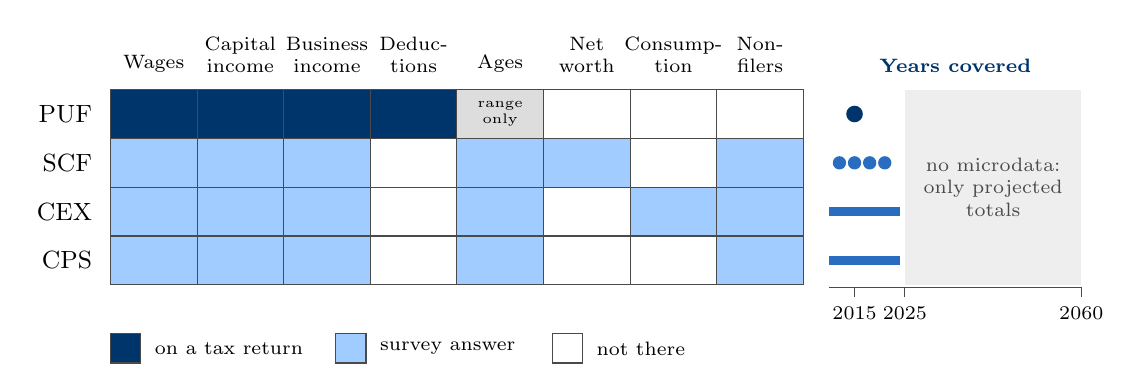
\begin{tikzpicture}[x=1.1cm, y=0.62cm]
    % column labels
    \foreach \lab [count=\i] in {Wages, {Capital\\income}, {Business\\income}, {Deduc-\\tions},
        Ages, {Net\\worth}, {Consump-\\tion}, {Non-\\filers}} {
      \node[font=\scriptsize, align=center, anchor=south] at (\i-0.5, 0.15) {\lab};
    }
    % rows: F = on a tax return, P = survey answer, N = not there
    \foreach \lab/\codes [count=\j] in {
        PUF/{cF,cF,cF,cF,cN,cN,cN,cN},
        SCF/{cP,cP,cP,cN,cP,cP,cN,cP},
        CEX/{cP,cP,cP,cN,cP,cN,cP,cP},
        CPS/{cP,cP,cP,cN,cP,cN,cN,cP}} {
      \node[font=\small, anchor=east] at (-0.1, -\j+0.5) {\lab};
      \foreach \c [count=\i] in \codes {
        \draw[\c, draw=yalegrey] (\i-1, -\j) rectangle (\i, -\j+1);
      }
    }
    % the PUF has the primary filer's age range only, and for most records
    \fill[yalelightgrey] (4,-1) rectangle (5,0);
    \draw[yalegrey] (4,-1) rectangle (5,0);
    \node[font=\tiny, align=center] at (4.5,-0.5) {range\\only};
    % legend
    \begin{scope}[shift={(0,-5.6)}]
      \draw[cF, draw=yalegrey] (0,0) rectangle (0.35,0.6);
      \node[font=\scriptsize, anchor=west] at (0.4,0.3) {on a tax return};
      \draw[cP, draw=yalegrey] (2.6,0) rectangle (2.95,0.6);
      \node[font=\scriptsize, anchor=west] at (3.0,0.3) {survey answer};
      \draw[cN, draw=yalegrey] (5.1,0) rectangle (5.45,0.6);
      \node[font=\scriptsize, anchor=west] at (5.5,0.3) {not there};
    \end{scope}

    % Click 2: which years each source covers, on a line from 2010 to 2060
    \onslide<2>{
    \begin{scope}[shift={(8.3,0)}, x=0.064cm]
      \node[font=\scriptsize\bfseries, text=yaleblue, anchor=south] at (25,0.15) {Years covered};
      % no microdata after the last survey year
      \fill[yalelightgrey!50] (15,-4.0) rectangle (50,0);
      \node[font=\scriptsize, align=center, text=yalegrey] at (32.5,-2) {no microdata:\\only projected\\totals};
      % PUF: 2015 only
      \fill[yaleblue] (5,-0.5) circle (3pt);
      % SCF: every third tax year
      \foreach \yr in {2012,2015,2018,2021} \fill[yalemid] (\yr-2010,-1.5) circle (2.4pt);
      % CEX and CPS: every year
      \draw[yalemid, line width=3pt] (0,-2.5) -- (14,-2.5);
      \draw[yalemid, line width=3pt] (0,-3.5) -- (14,-3.5);
      % axis under the last row
      \draw[yalegrey] (0,-4.05) -- (50,-4.05);
      \foreach \yr in {2015, 2025, 2060} {
        \draw[yalegrey] (\yr-2010,-4.05) -- (\yr-2010,-4.25);
        \node[font=\scriptsize, anchor=north] at (\yr-2010,-4.25) {\yr};
      }
    \end{scope}
    }
  \end{tikzpicture}

  \vspace{0.6em}
  No source has everything, and only one year has tax returns.
  \slidenote{Simplified. Years are tax years.}
\end{frame}

\begin{frame}{Why can't we just combine them?}
  \begin{itemize}
    \item \textbf{Different units.} Surveys count households; returns count tax units.
          One household can hold several returns, and some people file none.
    \vspace{0.6em}
    \item \textbf{Different definitions.} A return caps capital losses at \$3,000;
          survey wages are counted before pre-tax deductions.
    \vspace{0.6em}
    \item \textbf{Different measurement.} Small amounts go unreported: of every 100 couples,
          48 show interest on their returns, but only 21 tell the SCF they have any.
  \end{itemize}
  \slidenote{Interest: married couples with wages of \$75--200k, 2015 PUF and 2016 SCF (tax year 2015), weighted.}
\end{frame}

\begin{frame}{The task}
  \centering
  \vspace{1.5em}
  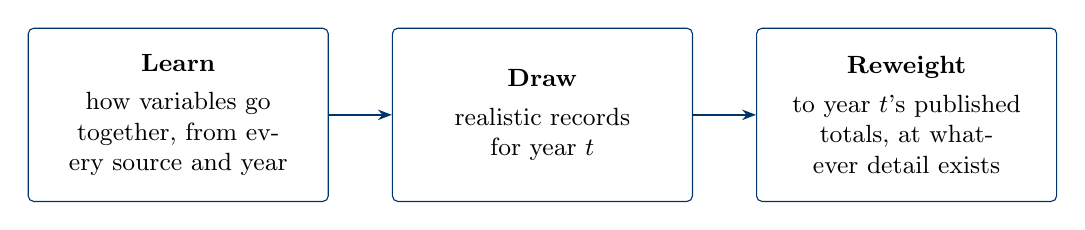
\begin{tikzpicture}
    \node[box, text width=3.6cm, minimum height=2.2cm, font=\small] (learn)
      {\textbf{Learn}\\[3pt] how variables go together, from every source and year};
    \node[box, text width=3.6cm, minimum height=2.2cm, font=\small, right=0.8cm of learn] (draw)
      {\textbf{Draw}\\[3pt] realistic records for year $t$};
    \node[box, text width=3.6cm, minimum height=2.2cm, font=\small, right=0.8cm of draw] (hit)
      {\textbf{Reweight}\\[3pt] to year $t$'s published totals, at whatever detail exists};
    \draw[arr] (learn) -- (draw);
    \draw[arr] (draw) -- (hit);
  \end{tikzpicture}
\end{frame}

\fi

\end{document}
